\section{Recursive Environment Evolution: Examples and Validation}
\label{app:synthesis}

The following cases illustrate how composition combines parent goals and how reconstruction turns the resulting reference graph into an executable task. Parent goals and observations are summarized for readability; generated requests and reference answers are reproduced in full.

\subsection{Composing goals with shared evidence}
\label{app:composition-case}

\begin{systembox}{Case 1 \quad Kong control-plane monitoring}
\textbf{Environment.} Control planes with routes and services, and groups of member control planes.

\casepart{Parent tasks and DAG transformation}
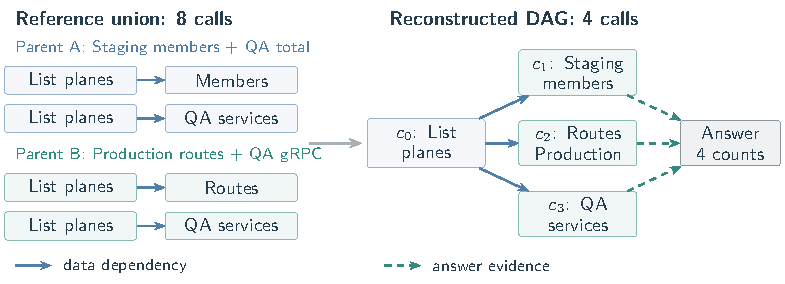
\includegraphics[width=\linewidth]{figures/synthesis_case_kong.pdf}

The two parent graphs form an eight-call reference union. Reconstruction merges the four discovery calls into one and the two QA-service queries into one, preserving all four requested counts.

\casepart{Generated request}
Find the control plane group named 'Staging' and count how many member control planes belong to that group. Then find the control plane named 'Production' with cluster type 'k8s' and count how many routes it has. Next, find the control plane named 'QA' with cluster type 'hybrid' in the 'ap-south' region and count both how many services are deployed to it and how many of those services use the 'grpc' protocol. Return the member count for the Staging group, the route count for Production, the total service count for QA, and the gRPC service count for QA.

\casepart{Reference execution \normalfont\small (all calls; condensed observations)}
\begingroup
\setlength{\tabcolsep}{3pt}\renewcommand{\arraystretch}{1.13}
\begin{tabularx}{\linewidth}{@{}l>{\raggedright\arraybackslash}p{.52\linewidth}Y@{}}
\toprule
 & Tool call & Observation \\
\midrule
$c_0$ & \texttt{list\_control\_planes()} & IDs: Staging group 2; Production/k8s 1; QA/hybrid/ap-south 5. \\
$c_1$ & \texttt{list\_control\_plane\_group\_memberships}\newline\texttt{(groupId=2)} & 2 member planes. \\
$c_2$ & \texttt{list\_routes(controlPlaneId=1)} & 30 routes. \\
$c_3$ & \texttt{list\_services(controlPlaneId=5)} & 10 services; 6 use gRPC. \\
\bottomrule
\end{tabularx}
\endgroup

\casepart{Reference answer and validation}
\noindent\begin{minipage}[t]{.64\linewidth}
\vspace{0pt}
\begin{lstlisting}[style=casejson]
{
  "staging_group_member_count": 2,
  "production_route_count": 30,
  "qa_total_service_count": 10,
  "qa_grpc_service_count": 6
}
\end{lstlisting}
\end{minipage}\hfill\begin{minipage}[t]{.32\linewidth}
\vspace{3pt}\raggedright
\textbf{State:} unchanged.\par\smallskip
\textbf{Passed:} execution, checker/replay, DAG checks, and both semantic reviews.
\end{minipage}
\end{systembox}
% Record: tc_kong_konnect_mcp_server:full:0002; parents S0003/S0015.
% Full parent requests, source node mappings and checker controls: evidence/cases/kong_case.json.
\begingroup\small
\refstepcounter{figure}\label{fig:composition-example}
\noindent\textbf{Figure \thefigure: Shared evidence across composed goals.} One discovery result supports three read branches; one service list answers both QA questions. The recorded execution is sequential.
\endgroup

\clearpage
\subsection{Pruning unused calls and restoring state order}
\label{app:reconstruction-case}

\begin{systembox}{Case 2 \quad Documentation refresh and search}
\textbf{Environment.} Documentation sources with crawl, indexing, and search operations.

\casepart{Parent tasks and DAG transformation}
Parent A refreshes the sources, counts enabled docs, and searches for ``hooks.'' Parent B refreshes the same sources, reports enabled docs and index size, and searches for ``error.''

\smallskip
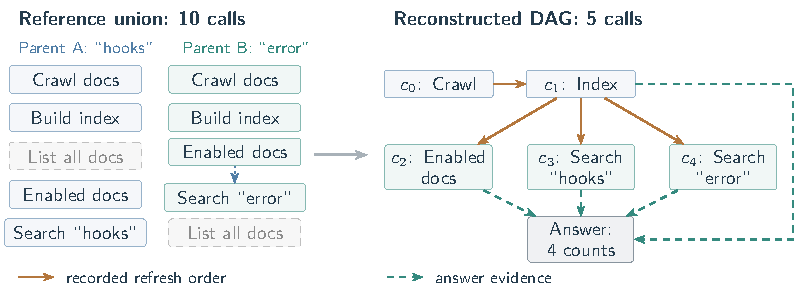
\includegraphics[width=\linewidth]{figures/synthesis_case_docs.pdf}

Reconstruction shares the crawl, index, and enabled-source calls, retains both searches, and removes the two \texttt{list\_all\_docs} calls (gray): their outputs add no requested result. The final DAG records refresh-before-query order. The dotted source edge is the only recorded candidate edge.

\casepart{Generated request}
Refresh the documentation search system by crawling all enabled documentation sources and rebuilding the search index. Then verify the system is working by checking how many documentation sources are currently enabled and indexed, and test the search functionality by querying for both 'hooks' and 'error'. Report the total number of enabled docs, total index entries created, and the number of search results found for each query term.

\casepart{Reference execution \normalfont\small (all calls; condensed observations)}
\begingroup
\setlength{\tabcolsep}{3pt}\renewcommand{\arraystretch}{1.13}
\begin{tabularx}{\linewidth}{@{}l>{\raggedright\arraybackslash}p{.52\linewidth}Y@{}}
\toprule
 & Tool call & Observation \\
\midrule
$c_0$ & \texttt{crawl\_docs()} & Enabled sources crawled. \\
$c_1$ & \texttt{build\_index()} & 10 docs indexed; 224 entries. \\
$c_2$ & \texttt{list\_enabled\_docs()} & 10 docs; all enabled, crawled, and indexed. \\
$c_3$ & \texttt{search\_docs(query='hooks')} & 2 matches. \\
$c_4$ & \texttt{search\_docs(query='error')} & 0 matches. \\
\bottomrule
\end{tabularx}
\endgroup

\casepart{Reference answer and validation}
\noindent\begin{minipage}[t]{.62\linewidth}
\vspace{0pt}
\begin{lstlisting}[style=casejson]
{
  "enabled_docs_count": 10,
  "index_entries_created": 224,
  "hooks_search_results": 2,
  "error_search_results": 0
}
\end{lstlisting}
\end{minipage}\hfill\begin{minipage}[t]{.34\linewidth}
\vspace{3pt}\raggedright
\textbf{State:} 10 docs updated; 24 pages and 224 index rows added.\par\smallskip
\textbf{Passed:} execution, checker/replay, DAG checks, and both semantic reviews.
\end{minipage}
\end{systembox}
% Record: tc_document_management_server:full:0006; parents S0009/S0010.
% Correspondences are inferred by matching operations, not a stored candidate-to-final node map.
% Recorded state order does not imply every reverse execution would fail.
\begingroup\small
\refstepcounter{figure}\label{fig:reconstruction-case}
\noindent\textbf{Figure \thefigure: Pruning and reconstruction.} Ten reference calls become five. Reconstruction also adds ordering edges, so the result is not a strict subgraph; the edges express the requested refresh order rather than a minimality guarantee.
\endgroup

\clearpage
\subsection{Execution and quality gates}
\label{app:synthesis-gates}

Table~\ref{tab:synthesis-gates} defines the acceptance checks. Failures trigger feedback and repair, with at most three generation attempts per candidate. Each attempt starts from a reset environment.

\begin{table}[H]
\centering\small
\caption{Quality gates and their acceptance conditions.}
\label{tab:synthesis-gates}
\renewcommand{\arraystretch}{1.17}
\begin{tabularx}{\linewidth}{@{}>{\raggedright\arraybackslash}p{.19\linewidth}Y@{}}
\toprule
Gate & Acceptance condition \\
\midrule
Plan validity & Allowed tools, valid arguments and unique call IDs; references resolve to earlier observations. \\
DAG consistency & One node per call plus an answer node; acyclic forward edges consistent with references and execution. State-order edges require evidence of a relevant state change. \\
Execution & Calls and answer computation succeed; tool contracts and database integrity hold. Contract-marked mutations change state. \\
Checker and replay & The checker accepts the reference and rejects corrupted answers and applicable state controls. Fresh-state replay reproduces the answer and required changes without unexpected mutations. \\
Semantic review & Both reviews pass all six criteria, cover both parents' outcomes, and leave no unresolved issue. \\
\bottomrule
\end{tabularx}
\end{table}

\begin{systembox}{Six semantic review criteria}
\setlength{\tabcolsep}{0pt}\renewcommand{\arraystretch}{1.2}
\begin{tabularx}{\linewidth}{@{}>{\bfseries\raggedright\arraybackslash}p{.32\linewidth}Y@{}}
Task fulfillment & Does execution accomplish the generated request? \\
Answer completeness & Does the answer include every requested result? \\
Parent preservation & Are both parents' functional outcomes retained? \\
Workflow coherence & Do the operations serve one coherent task? \\
State consistency & Do state claims agree with execution and the final database? \\
Justified repetition & Does each repeated call add information, observe changed state, or serve a distinct purpose? \\
\end{tabularx}
\smallskip
\textit{Condensed from the review protocol; every criterion requires supporting evidence.}
\end{systembox}

\noindent\textbf{Review setup and coverage.} The generator and both reviewers use Claude Sonnet 4.6. Review 2 sees no earlier verdict and runs only after Review 1 passes. All 2,581 accepted tasks pass both reviews; 2,037 also carry explicit question-DAG validation, while 544 follow the earlier policy.

\begin{figure}[H]
\centering
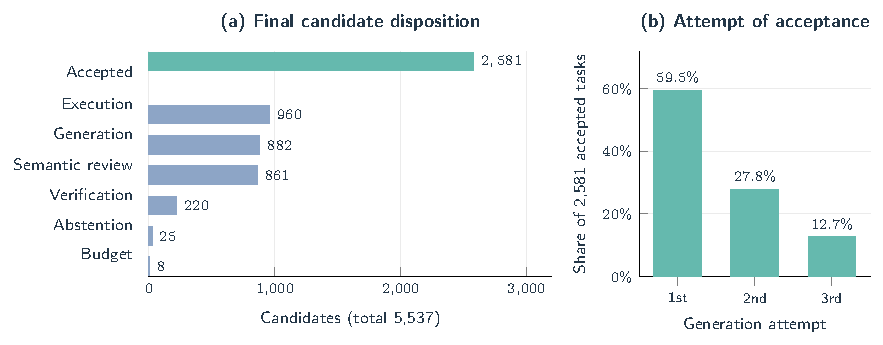
\includegraphics[width=.91\linewidth]{figures/synthesis_gate_outcomes.pdf}
\caption{\textbf{Candidate outcomes and repair.} Left: one final disposition per candidate, assigned to its last recorded stage, rather than a sequential filtering funnel. Right: successful attempt among 2,581 accepted tasks (46.61\%). Of these, 1,045 (40.49\%) pass after repair: 717 on attempt 2 and 328 on attempt 3.}
\label{fig:synthesis-gate-outcomes}
\end{figure}

\FloatBarrier

\clearpage
\subsection{Dataset profile and measurement definitions}
\label{app:synthesis-statistics}

The synthesis batch starts from 10,860 seeds across 598 environments and evaluates 5,537 two-parent reference unions. It yields 2,581 accepted tasks across 539 environments; 835 require state changes. The batch instantiates one composition round of the recursive procedure. Multi-round effects are left to the construction ablations below.

\begin{table}[H]
\centering\small
\caption{Mean reference structure before and after synthesis. The matched baseline is the mean of each accepted task's two parents, not their combined workload.}
\label{tab:synthesis-profile}
\setlength{\tabcolsep}{5pt}
\begin{tabularx}{\linewidth}{@{}Yrrrr@{}}
\toprule
Metric & All seeds & Matched parents & Accepted & Change \\
\midrule
Tool calls & 4.535 & 3.978 & 4.757 & +19.6\% \\
Distinct tools & 3.191 & 2.842 & 2.953 & +3.9\% \\
Answer fields & 3.623 & 3.483 & 5.478 & +57.3\% \\
\bottomrule
\end{tabularx}
\end{table}

\paragraph{Metric definitions.}
Tool calls count operations in the seed reference or reconstructed plan; distinct tools count unique tool names within that reference; answer fields count top-level dictionary keys. For task $i$, the matched baseline is $b_i=[m(p_{i1})+m(p_{i2})]/2$, and relative change is $100(\bar m/\bar b-1)$. A reused parent contributes once per descendant. The answer-field comparison excludes three non-dictionary seed answers and one affected parent pair, leaving 2,580 matched tasks. The corresponding mean over all 2,581 accepted tasks is 5.477, as shown in Figure~\ref{fig:task-statistics}.

\paragraph{Interpretation.}
The matched comparison measures how an accepted task differs from its own parents; the unconditional distributions describe the full seed and accepted populations. Both describe reference structure, rather than measured solver difficulty or training gains. The examples show recorded dependencies and request-consistent state order, without claiming minimal plans or measured parallel speedup. Reconstruction may merge, remove, or add operations and edges; strict-subgraph and counterfactual edge tests were not enabled in this batch.

\subsection{Construction ablations and structural measurements}

The construction experiment uses the same backend pool and generator for every row of Table~\ref{tab:construction-ablation}. Equal synthesis-budget runs measure accepted-task yield and cost per accepted task. Equal accepted-data runs measure downstream training utility with the same outcome-only MA learner. If a variant cannot supply the common task count, the experiment reduces all arms to their common feasible count or reports that arm separately; duplicating samples does not establish equal diversity.

\begin{table}[ht]
\centering\small
\caption{Construction ablations. Yield is accepted tasks per fixed generation budget; success is held-out task success after training on equal accepted-task counts. All values are pending.}
\label{tab:construction-ablation}
\begin{tabularx}{\linewidth}{Ycccc}
\toprule
Training-task source & Yield & Cost/task & Goals/task & Success (\%) \\
\midrule
Original seed tasks & \pending & \pending & \pending & \pending \\
Direct synthesis & \pending & \pending & \pending & \pending \\
One-round composition & \pending & \pending & \pending & \pending \\
Recursive serial-only & \pending & \pending & \pending & \pending \\
Recursive parallel-only & \pending & \pending & \pending & \pending \\
Full recursive composition & \pending & \pending & \pending & \pending \\
\bottomrule
\end{tabularx}
\end{table}

Planned structural measurements use the accepted reference: functional goals per task, required dependency relations, verified independent goal pairs, and shared evidence sources. We also report reference calls, but do not equate call count with task difficulty or rollout length. Lineage depth, ancestor count, reference-graph depth, and policy critical-path rounds are separate fields. Read-only independence must pass the order-validation procedure below before it is used for decomposition rewards.

\section{Runtime Interface and Information Boundary}
\label{app:runtime}

\subsection{Actions and execution semantics}

Table~\ref{tab:actions} describes the implemented orchestration actions. A worker is registered with a role description and a permitted tool subset. Single assignment is synchronous; batch assignment launches workers concurrently and returns after their results join. Worker reasoning can overlap, while tool state operations commit under a transaction lock. The observed implementation does not expose a general direct-tool action to the orchestrator, and its completion protocol requires at least one delegation. The manuscript therefore does not claim that it learns to choose between zero-worker execution and delegation.

\begin{table}[ht]
\centering\small
\caption{Orchestration action interface. Exact prompt and parser versions must accompany the final run manifest.}
\label{tab:actions}
\begin{tabularx}{\linewidth}{lY}
\toprule
Action & Required information and effect \\
\midrule
\texttt{create\_subagent} & Name, system prompt, and allowed tool names; registers a frozen-model worker. \\
\texttt{assign\_task} & Worker name and subtask prompt; executes one assignment and returns its result. \\
\texttt{assign\_tasks} & List of assignments; permits concurrent worker inference and joins their returns. \\
\texttt{submit\_answer} & Final answer in the required format; triggers completion and verification. \\
\bottomrule
\end{tabularx}
\end{table}

The paired MA baselines share tool schemas, role prompts, worker histories, truncation rules, and parser behavior. Serializing the trained policy replaces batch concurrency with ordered execution of its requested assignments, preserves output ordering, and logs any state-sensitive divergence. It is an inference intervention, not a new policy trained on serial traces. For stateful tasks, differences in returned observations can also change later decisions, so the intervention is not assumed to alter time alone.

\subsection{Visible and privileged information}

\begin{table}[ht]
\centering\small
\caption{Information boundary during an episode. Reward reports are not returned as observations.}
\label{tab:visibility}
\begin{tabularx}{\linewidth}{Yccc}
\toprule
Information & Orchestrator & Worker & Reward service \\
\midrule
User request & Yes & Assigned content & Yes \\
Allowed tool descriptions & Yes & Permitted subset & Yes \\
Actual tool/worker returns & Returned content & Own context & Logged content \\
Reference plan and expected answer & No & No & Yes \\
Verifier code and process contract & No & No & Yes \\
Milestone and reward-component scores & No & No & Yes \\
\bottomrule
\end{tabularx}
\end{table}

A leakage audit inspects the actual rendered requests and tool descriptions, not just source templates. The audit checks for reference answers, serialized reference graphs, verifier diagnostics, and accidental hidden-file access. Final train/test manifests also record normalized task text and source lineage. Tasks descending from the same seed family must be grouped before splitting; an environment-disjoint evaluation additionally groups all tasks from an environment. These checks are required for final experiments and are not represented as already completed by the existence of an import file.

\subsection{Event log and critical-path reconstruction}

Execution cost is a diagnostic, not a reward component in Eq.~\ref{eq:reward}. Let $w(v)=1$ for each orchestrator or worker generation event and zero for other events. With only causal parents retained, define
\begin{equation}
 d(v)=w(v)+\max_{u\in\operatorname{pa}_{\rm causal}(v)}d(u),\qquad C(\tau)=\max_{v\in G_\tau}d(v).
 \tag{B.1}\label{eq:critical-path}
\end{equation}
An empty maximum is zero. Edges representing only the serialized database commit order are excluded. The resulting logical model rounds omit tool latency and generation length; wall-clock time and total tokens are reported separately.


Every event needs an episode ID, event ID, actor, event kind, causal parent IDs, and any transaction-order parent. Model-generation events carry prompt/completion token counts and timing; tool events additionally record tool identity, normalized arguments, observation, status, and assignment ownership. Assignment start/end events connect worker execution to its returned result. Logs must preserve ordering and parent references so Eq.~\ref{eq:critical-path} can be recomputed independently of the reward hook.

For an illustrative fork--join execution, one orchestrator generation precedes two independent worker branches of lengths three and five, followed by one integration generation. Its critical path is $1+\max(3,5)+1=7$ model rounds; serializing those branches gives $1+3+5+1=10$. Both perform ten generations. These are arithmetic examples, not measured latency or accuracy results. Tool latency and generation length can make the corresponding wall-clock ratio very different from $10/7$.

\section{Process Reward: Matching Rules and Applicability}
\label{app:process}

\subsection{Tool and answer matching}

A reference milestone specifies a tool, canonical arguments, an observation digest, and supported aliases. Arguments are compared after filling declared defaults and applying explicitly listed environment-specific normalization rules. Observations are JSON-canonicalized when possible and hashed. Only successful matching events contribute coverage, with each reference milestone counted once. Information dependencies require available predecessor evidence; state dependencies also use execution order.

The recorded retrieval-window exception removes only \texttt{limit}, \texttt{max\_results}, \texttt{per\_page}, \texttt{page\_size}, and \texttt{show} from argument comparison. Both calls must be non-mutating; the actual observation must be nonempty JSON shorter than 12,000 characters and must retain the reference observation digest. This does not accept arbitrary broader queries or semantic paraphrases.

The answer score in Eq.~\ref{eq:answer-coverage} uses top-level key--value rows. A missing reference key receives zero; an extra candidate key increases the precision denominator. A scalar or structured value requires equality. List elements are matched one-to-one without reusing an element, and fractional list coverage contributes to the equivalent matched-row count. Empty or invalid submissions receive zero. Final binary acceptance remains governed by the task's answer/state checker.

\subsection{Allocation, delivery, and integration}

Independent-goal allocation is eligible only when the reference contains independent goal pairs, its milestones are non-mutating, and its order-proof record has three passing executions including a changed order. These tests establish eligibility for the supported scorer, not universal commutativity. Ambiguous reference occurrences do not receive guessed ownership.

Each credited goal must have one assignment owner. Repeated or empty instructions do not receive allocation credit. A legal exact attempt receives partial credit; a matched observation and a returned worker result provide full goal evidence. Pair scoring checks distinct ownership and causal independence of assignment boundaries, then discounts redundant or irrelevant allocation.

Answer-dataflow annotations connect supported goals to their source operands and final-answer components. Delivery checks whether the worker return contains the required raw evidence or a matching derived result. Integration checks the corresponding final-answer components and the whole answer. In Eq.~\ref{eq:process}, $S$ denotes allocation credit after delivery and integration adjustments. This notation absorbs the implementation's multiplicative integration adjustment; it does not add a reward component or remove the check for missing results. $D$ is mean supported-goal delivery.

\subsection{Fallbacks and implementation binding}

Stateful tasks, missing answer-dataflow support, or ambiguous references cannot be assigned the supported independent-goal formula unconditionally. The documented matching implementation uses conservative progress based on covered milestones, satisfied dependencies, productive assignments, returned evidence, and nonredundant tool events. Missing or mismatched mandatory reference artifacts are integrity errors, rather than policy failures.

The revised main text specifies the supported-branch weights and the cost-free reward from the author's annotated draft. Historical development formulas use different weights and must not be reused as the final fallback specification. \drafttodo{Bind the final reward module and configuration hashes, exact fallback coefficients, row-matching edge cases, and the number of tasks supported by each branch before reporting training results.}

\subsection{Outcome priority}

Under Eq.~\ref{eq:reward}, $O=1$ and $P\geq0$ imply $R_{\rm success}\geq1$. For a failed trajectory, $O=0$ and $P\leq1$ imply $R_{\rm failure}\leq\lambda_p=0.3$. Every verified success therefore outranks every failure under this scalar reward. This property assumes a correct outcome evaluator and bounded process scores; it does not guarantee policy convergence or an improvement in success rate.

\section{Optimization and Configuration}
\label{app:training}

Let $\mathcal T_i$ denote orchestrator-generated token positions in rollout $i$, and $\rho_{it}(\theta)$ the ratio of current to behavior-policy token probabilities under the recorded context. The clipped GRPO policy term can be written
\begin{equation}
 J(\theta)=\mathbb E\!\left[\frac1G\sum_{i=1}^{G}\frac1{|\mathcal T_i|}
 \sum_{t\in\mathcal T_i}\min\!\left(\rho_{it}A_i,
 \operatorname{clip}(\rho_{it},1-\epsilon_l,1+\epsilon_h)A_i\right)\right]
 -\beta\mathcal K(\theta).
 \tag{D.1}
\end{equation}
Here $\mathcal K$ denotes the configured KL regularizer. This expression states the policy-ratio objective; exact loss aggregation, KL estimator, and clipping settings must be bound to the final trainer configuration. Worker completions, tool returns, and other observations are excluded from $\mathcal T_i$. Their probability is not optimized through the orchestrator loss.

\begin{table}[ht]
\centering\small
\caption{Working training configuration. Earlier recorded settings are distinguished from the revised reward specification; the final run binding remains pending.}
\label{tab:configuration}
\begin{tabularx}{\linewidth}{YY}
\toprule
Setting & Recorded value \\
\midrule
Backbone & Qwen3-8B \\
Orchestrator initialization & Single-agent checkpoint (recorded rollout 1550) \\
Worker initialization/update & Same checkpoint / frozen \\
Imported training set & 2,577 tasks in the earlier import; final manifest pending \\
Optimization & GRPO; outcome + process reward \\
Task batch / rollouts per task & 16 / 8 \\
Training duration & 3 epochs planned; 483 updates planned \\
Process coefficient $\lambda_p$ & 0.3 \\
Cost in training reward & None \\
KL handling & Enabled in recorded process flags; coefficient to be frozen \\
Completion protocol & At least one delegation required \\
\bottomrule
\end{tabularx}
\end{table}

The revised reward weights follow the annotated manuscript; the earlier runtime snapshot supports the recorded interaction and masking behavior. These sources do not establish a completed run under the revised specification. Final experiments must bind model/checkpoint hashes, dataset/split hashes, reward code and configuration, completed updates, learning rate, KL estimator and coefficient, clipping bounds, loss aggregation, decoding, truncation, worker limits, timeouts, hardware, and compute. The 2,581 synthesized records and the earlier 2,577-record import require a separate ID-level reconciliation.

\section{Evaluation Manifest and Statistical Protocol}
\label{app:benchmarks}

\subsection{Benchmark identity and adapters}

Table~\ref{tab:benchmark-manifest} fixes the intended identities while exposing unresolved versions. The first four are supported by the project's evaluation inventory; Terminal-Bench 2.0 is selected from an existing experiment registration. BFCL and $\tau^2$-Bench extend coverage based on the earlier blueprint and related tool-use evaluations. This seven-column roster is a working choice, not an assertion that the author has frozen all seven protocols.

\begin{table}[ht]
\centering\footnotesize
\caption{Working benchmark manifest. Every final score requires a dataset revision, evaluator commit, subset manifest, and decoder configuration.}
\label{tab:benchmark-manifest}
\begin{tabularx}{\linewidth}{lYY}
\toprule
Benchmark & Metric and purpose & Version/adapter boundary \\
\midrule
WideSearch & Official item F1 as primary; whole-case accuracy separately & ByteDance-Seed/WideSearch; split and scorer commit pending. \\
DeepPlanning & Official \texttt{avg\_acc}; report task-family breakdown & Pin release, travel/shopping subsets, and aggregation rule. \\
MCP Atlas & Official claim-rubric pass rate; freeze coverage threshold & scaleapi/mcp-atlas; distinguish available-service subset from full benchmark. \\
Toolathlon & Official task success & Toolathlon-GYM adapter; pin task set, services, and evaluator. \\
BFCL multi-turn & Official multi-turn accuracy & Freeze BFCL version and category aggregation; do not mix v3/v4 scores. \\
$\tau^2$-Bench & Official task success at the declared trial protocol & Pin verified/original version, domains, user simulator, and repetitions. \\
Terminal-Bench 2.0 & Official task resolution & Pin 2.0 task revision and harness; do not substitute 2.1 or later scores. \\
\bottomrule
\end{tabularx}
\end{table}

The official project entry points include \href{https://github.com/ByteDance-Seed/WideSearch}{ByteDance-Seed/WideSearch}, \href{https://github.com/scaleapi/mcp-atlas}{scaleapi/mcp-atlas}, \href{https://github.com/eigent-ai/toolathlon_gym}{eigent-ai/toolathlon\_gym}, and \href{https://github.com/harbor-framework/terminal-bench-2}{harbor-framework/terminal-bench-2}. These identify resources, not immutable experimental versions. A main-table result must reference a frozen revision and explicit metric key. Source adapters may normalize tool-call syntax but must preserve task semantics, evaluator behavior, and information access.

\subsection{Paired estimates and costs}
\label{app:statistics}

The primary unit is the task. Within each benchmark, every method attempts the same instances under paired evaluation seeds and identical initial states where the benchmark permits deterministic reset. Multiple rollout seeds on a task are averaged before task-level aggregation. The proposed uncertainty protocol uses 10,000 paired bootstrap resamples of task IDs and reports percentile 95\% intervals for scores and method differences. For repeated training runs, training-seed variation is additionally reported and resampled hierarchically; evaluation-only intervals must not be described as training uncertainty. The final number of training and evaluation seeds remains to be declared.

For a benchmark with native domain weighting, the bootstrap preserves that aggregation rather than replacing it with a pooled task average. No average over heterogeneous benchmark metrics is used in the main table. Whole-task correctness is distinct from field-level accuracy, partial credit, or process reward. If significance tests are added, their hypotheses and multiplicity correction must be specified before interpreting many pairwise contrasts.

All-episode mean cost includes failed and timed-out attempts. We also report wall-clock median and 90th percentile, timeout frequency, total input/output tokens across every model, tool attempts, and peak active workers. Latency is measured from episode start to terminal answer or timeout under declared hardware and concurrency conditions. Environment reset and queueing costs are separately logged with an explicit inclusion policy. A both-success subset can diagnose speed differences but is secondary because conditioning on success can favor different populations.

Infrastructure exceptions, such as unavailable services or reset failures, are recorded separately from a valid trajectory that fails verification. A rerun policy must use the same inputs and count all replacement attempts in the audit. Persistent missing infrastructure is reported as coverage loss, not silently removed to improve a score. The final run ledger records attempted, completed, failed, timed-out, rerun, and unavailable episodes for each method.

\section{Extended Results and Behavior Audits}
\label{app:extended-results}

\begin{table}[ht]
\centering\small
\caption{Per-benchmark efficiency record for each method. Duplicate this block for Base, Single-agent, Multi-agent, AWM, EnvScaler, and MAW when results arrive. Values remain pending. Latency quantiles include the declared timeout handling.}
\label{tab:efficiency}
\begin{tabularx}{\linewidth}{Yccccc}
\toprule
Benchmark & Mean $C$ & Tokens (k) & Time p50 & Time p90 & Timeouts (\%) \\
\midrule
WideSearch & \pending & \pending & \pending & \pending & \pending \\
DeepPlanning & \pending & \pending & \pending & \pending & \pending \\
MCP Atlas & \pending & \pending & \pending & \pending & \pending \\
Toolathlon & \pending & \pending & \pending & \pending & \pending \\
BFCL multi-turn & \pending & \pending & \pending & \pending & \pending \\
$\tau^2$-Bench & \pending & \pending & \pending & \pending & \pending \\
Terminal-Bench 2.0 & \pending & \pending & \pending & \pending & \pending \\
\bottomrule
\end{tabularx}
\end{table}

Behavior audits use held-out MAW tasks with reference annotations. Coverage is the matched-goal fraction, delivery is the mean supported-goal delivery score, and duplicate allocation is excess assignment ownership per attempted goal. We report the fraction and count of tasks supporting each metric, including the subset eligible for independent-goal scoring. External benchmarks without such annotations receive only their official outcome scores and available runtime metrics; MAW process scores are not retroactively inferred from benchmark answers.

\begin{table}[ht]
\centering\small
\caption{Failure taxonomy for trace review. Labels may co-occur; their rates are not assumed to sum to 100\%.}
\label{tab:failures}
\begin{tabularx}{\linewidth}{lY}
\toprule
Failure class & Auditable criterion \\
\midrule
Goal omission & A required subgoal has no supporting execution evidence. \\
Duplicate work & Multiple assignments repeat a goal without new evidence or a required retry. \\
Dependency misuse & A consumer executes without the prerequisite information or state. \\
Handoff failure & A worker obtains relevant evidence but its return omits the required content. \\
Integration failure & Available branch results are omitted or incorrectly combined in the final answer. \\
Worker execution & Delegation is appropriate but local tool choice, arguments, or reasoning fail. \\
Budget exhaustion & The episode reaches the common token, step, or time limit before completion. \\
Environment/checker error & Replay, state behavior, or evaluation is inconsistent with the declared task. \\
\bottomrule
\end{tabularx}
\end{table}

Case reports should include the task ID, visible request, selected tool descriptions, assignment prompts, relevant tool observations, worker returns, final answer, verifier outcome, and actual execution graph. A successful and an unsuccessful case from each principal structure slice should be selected by a declared sampling rule rather than chosen solely for visual appeal. The reference may be shown post hoc for analysis, clearly separated from policy-visible content. Annotators review goal omission, dependency, handoff, and integration evidence separately and record disagreements. The case-study counts and agreement measurements remain pending.

\section{Availability, Ethics, and Author Declarations}
\label{app:declarations}

\paragraph{Data and code availability.}
The planned research package contains environment/reset manifests, task provenance, synthesis and acceptance code, reward-side annotations, prompts, baseline adapters, training configurations, and per-task evaluation logs. Public release URLs and licenses have not yet been finalized. Access to hidden evaluation references must remain separated from solver-facing assets. \drafttodo{Add the frozen repository commit, release location, license inventory, and access conditions.}

\paragraph{Ethics and limitations of use.}
Synthetic tool environments can contain unrealistic assumptions or faulty checks. They should be executed in isolated sandboxes and reviewed for copied private data, credential-like strings, and unauthorized external side effects before release. The task concerns agent training rather than a human-subject experiment; this statement does not replace an institutional determination where one is required. The same orchestration capability can coordinate harmful actions, so deployment requires tool-specific permissions and monitoring beyond the training reward.

\paragraph{Author contributions, conflicts, and funding.}
\drafttodo{Authors must supply their CRediT contributions, conflict-of-interest declaration, and funding acknowledgments. No declaration of absence is inferred.}

\paragraph{AI assistance.}
AI assistance was used to analyze supplied writing examples, draft and edit manuscript text, organize experimental tables, and check LaTeX consistency. Numerical experimental results were not generated to fill missing measurements. The authors remain responsible for reviewing technical claims, references, and experimental reporting. This working disclosure must be checked against the applicable submission policy before submission; no venue-policy compliance is asserted here.
